\section{System design}\label{sec:sys}
This section gives a depiction of the operations designed in the smart contract and the interaction procedure between the components of our architecture. Moreover, we give some discussion about the system limitations. 
 
\subsection{Smart Contract}
Figure \ref{fig:data-structure} shows the data structure in the smart contract.
Each drone covers one or multiple WSNs and takes responsibility for a set of IoT devices in the WSNs, and each IoT device generates at most one offloading task at one time.
The task will be offloaded to a specific MEC server by smart contract through a drone.

It is assumed that $I$ is the set of public keys of $I(d)$ of each drone $d$, 
$G$ is the set of the public keys $G(m)$ of each IoT device $m$ and $P$ is the set of offloading policies where $p$ refers to the specific offloading rules to select the ``best" MEC server to offload tasks from IoT devices.
%$$I=\{I(d_1),I(d_2),...,I(d_n)\}$$
%$$G=\{G(m_1),G(m_2),...,G(m_n)\}$$
%$$Q=\{Q(s_1),Q(s_2),...,Q(s_n)\}$$
%$$P=\{p_1,p_2,...,p_n\}$$


\begin{figure}[t]
\centering
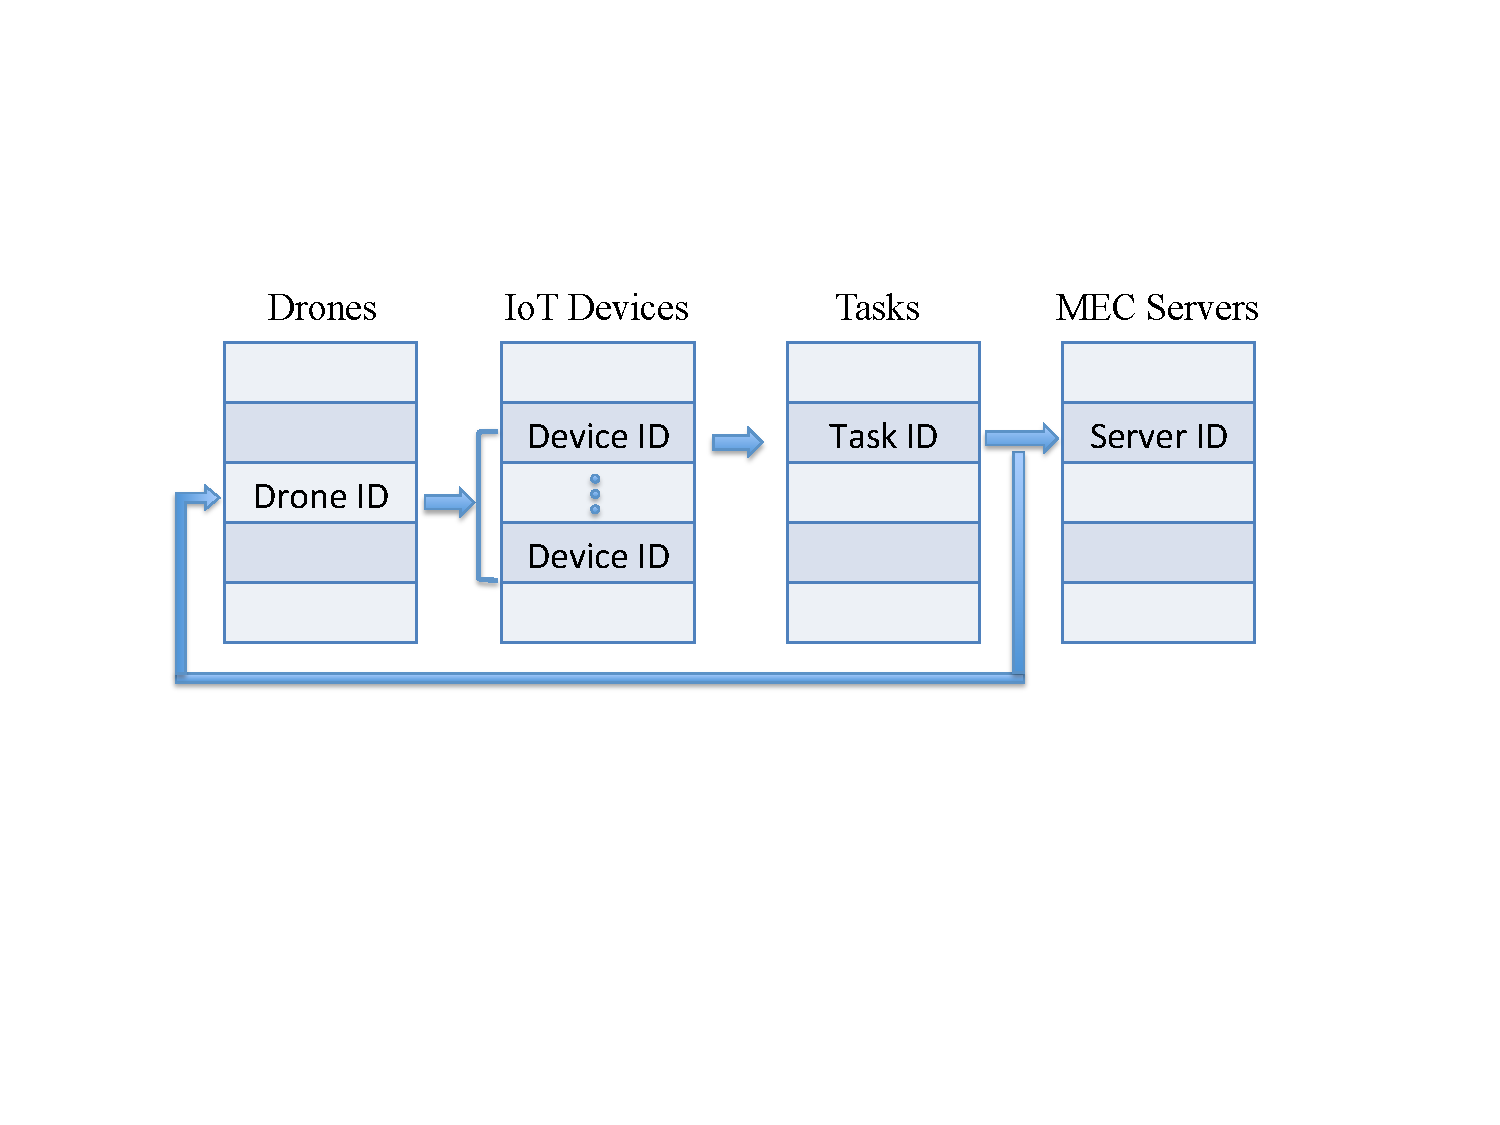
\includegraphics[width=3.3 in]{Fig/DataStructure.pdf}
\caption{Data Structure in the Smart Contract}
\label{fig:data-structure}
\end{figure}

In the smart contract,  the drones and IoT devices are identified in the offloading system by their public keys.
The order of components registration is depicted below.
First MEC servers are signed in by the operation $RegisterServer(Q(s))$, next the drones are joined by  $RegisterDrone(Q(s), I(d))$ iff drone $d$ is authorized by MEC server $s$.
After that, the IoT devices are registered by $RegisterDevice(I(d), G(m))$ iff drone $d$ is the offloading hub of device $m$. 
Besides, the tasks will be identified by their IDs.
The mapping from the drone to the IoT device is done by $AddDronetoDevice(I(d), G(m), Q(s), p)$ iff drone $d$ is the offloading hub of device $m$.
The offloading policy can be deployed into the smart contract by $AddOffloadingPolicy(I(d), G(m), Q(s), p)$, which determines how to choose the MEC server to offload.
When it needs to find the offloading hub of the specific IoT device, $QueryDrone(I(d))$ can be called.
$QueryOffloading(I(d), t, G(m), Q(s), p)$ is used to obtain the result of offloading task $t$ by executing offloading policy $p$.
It is worthy to mention that the fetching process does not incur any fee or latency, since drones obtain the information from the blockchain store directly, rather than use a transaction. 

% The operations defined in our smart contract are described as follows.
% \begin{itemize}
%\item $RegisterServer(Q(s))$: $Q^* \leftarrow Q \bigcup Q(s)$ for any MEC server $s$.
%\item $RegisterDrone(Q(s), I(d))$: $I^* \leftarrow I \bigcup I(d)$ iff drone $d$ is authorized by MEC server $s$.
%\item $RegisterDevice(I(d), G(m))$: $G^* \leftarrow G \bigcup G(m)$ iff drone $d$ is the offloading hub of device $m$. 
%\item $AddDronetoDevice(I(d), G(m))$: $G^* \leftarrow G \bigcup G(m)$ iff drone $d$ is the offloading hub of device $m$.
%\item $AddOffloadingPolicy(I(d), G(m), Q(s), p)$: $P^* \leftarrow P \bigcup p$ iff drone $d$ is the offloading hub of device $m$.
%\item $DeRegisterServer(Q(s))$: $Q^* \leftarrow Q \bigcap Q(s)$.
%\item $DeRegisterDrone(I(d))$: $I^* \leftarrow I \bigcap I(d)$.
%\item $DeRegisterDevice(G(m))$: $G^* \leftarrow G \bigcap G(m)$.
%\item $QueryDrone(I(d))$: returns the tuple $(d,U)$ where $U=\{u \in G, d$ is the offloading hub of device $u\}$. 
%\item $QueryOffloading(I(d), t, G(m), Q(s), p)$: returns the result of offloading task $t$ by executing offloading policy $p$.
%\end{itemize}


\subsection{Offloading Policy}
The offloading policy plays a crucial part as it determines which local MEC server would be performed the offloading computation task.
Currently, the design of offloading policies usually takes multiple factors into consideration together, such as the distance of the request device and the MEC server, the access and computation capacity of MEC servers, the security level of MEC servers, and the availability of wireless connection links, etc.
In this paper, we only consider some simple offloading policies as discussed in the following.

\subsubsection{The Random Policy}
When the drone has no prior knowledge about the MEC servers, the drone will choose randomly one MEC server to offload the task delivered from IoT devices.

\subsubsection{The Nearest Policy}
The drone will connect with the nearest available MEC server in the blockchain network, a miner node in Figure \ref{fig:network-arch}.
The nearest policy indicates that drones always find the nearest MEC server to offload the task from IoT devices.

\subsubsection{The Max Computing Capacity (MCC) Policy}
In max computing capacity policy, the drones always choose the MEC server with the maximum computing capacity to offload tasks.

\subsubsection{Smart Contract Policy}
 In our smart contract policy, it aims to find the best offloading MEC server with minimum latency.
 Since the scale of the blockchain network is so small, we assume that the consensus time is negligible or with little difference among different policies.
 Thus, we focus on the task transmission delay and computation offloading delay.
Given that $a_t$ is the data amount of offloading task $t$, $\bar{r}$ the average transmission rate, $b_t$ is the computation amount of offloading task and $\bar{c}$ the average computing capacity, the drone will choose the MEC server by the Nearest policy if $a_t/\bar{r}   >  b_t/\bar{c}$, otherwise by the MCC policy.




 
\subsection{System Interactions}
Figure \ref{fig:SmartContract} illustrates the interactions among the system components, which can be divided into three phases: establishing the blockchain network, signing the drones and IoT devices into the system, and executing the offloading operation for the tasks from IoT devices.

\begin{figure*}[t]
\centering
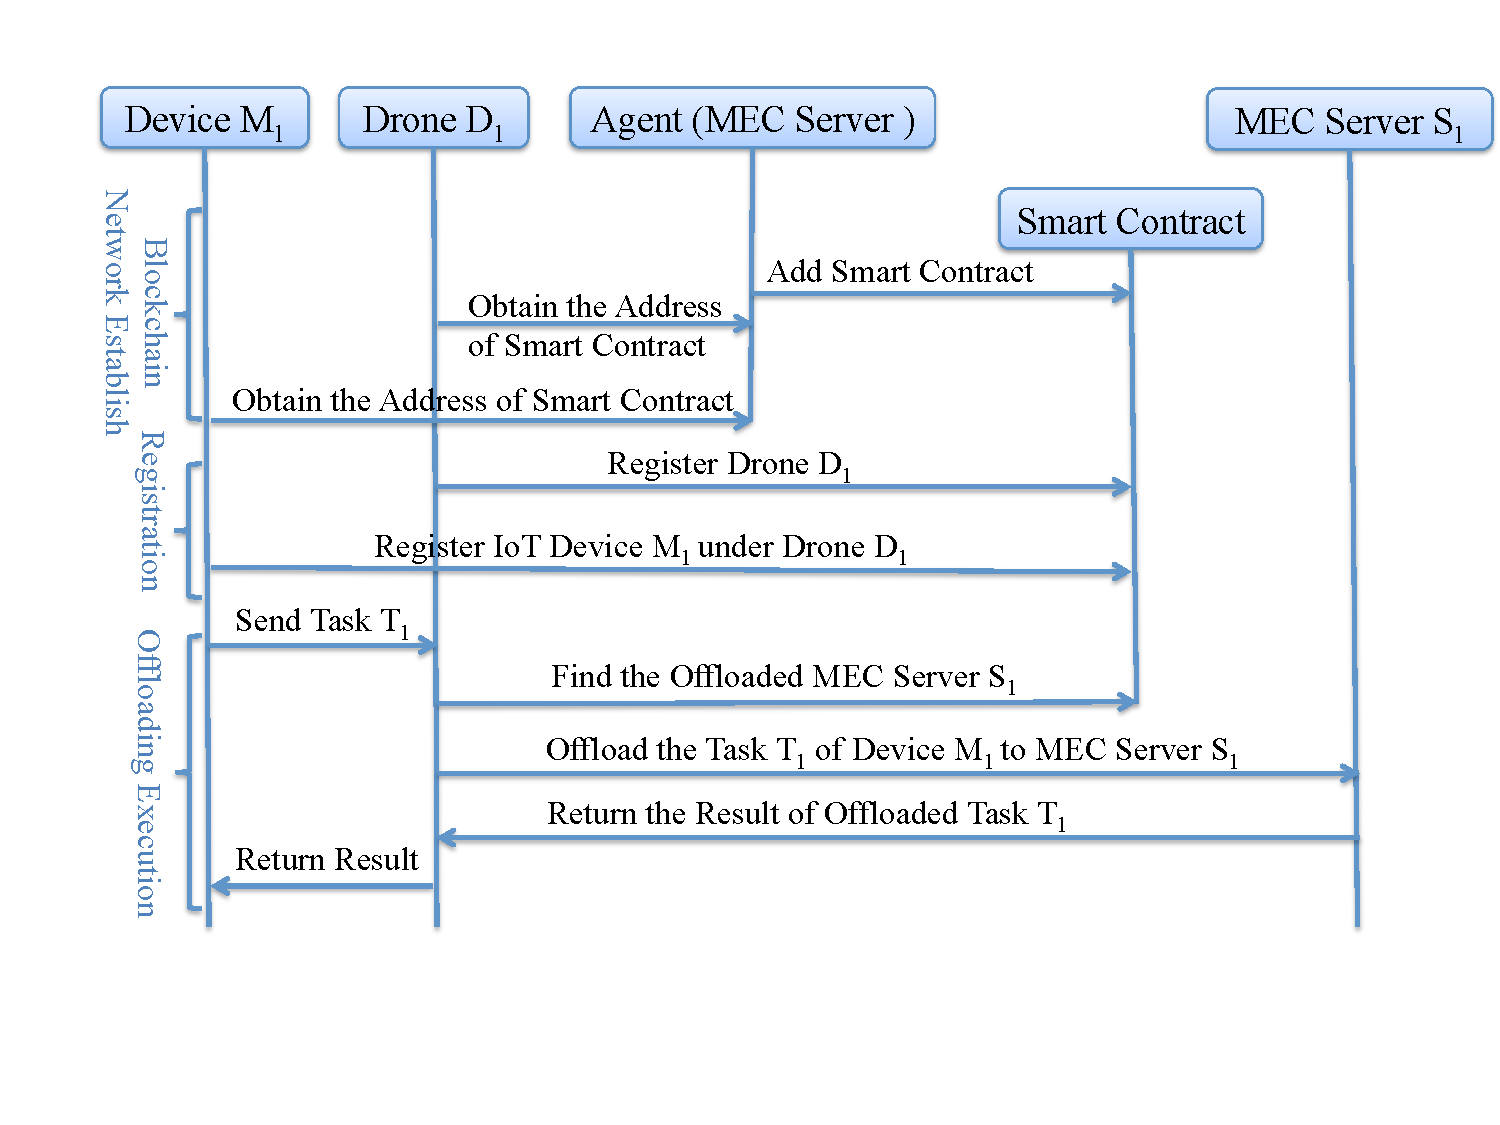
\includegraphics[width=4.5 in]{Fig/SmartContract.pdf}
\caption{Network Establishment, Registration and Offloading Execution}
\label{fig:SmartContract}
\end{figure*}

\subsubsection{Network Establishment}
 The blockchain network is established among the network of MEC servers in the beginning. 
Once the blockchain network is created, the agent node takes the responsibility to deploy the smart contract into the blockchain network. 
The smart contract defines all the operations of the offloading policy and it will generate an unique address to identify this smart contract when it is accepted by the blockchain network.
All components in the offloading system use that unique address to interact with the smart contract and execute the operations automatically designed in the smart contract.
 For example, all the drones in the system need to register as offloading hubs by interacting with the smart contract.

Figure \ref{fig:SmartContract}  shows how a drone interact with the address and query the Agent node. 
The offloading hub connects with several available MEC servers in the blockchain network, i.e., miner nodes.
 Each miner hosts a distributed copy of the blockchain to make all the operations to offloaded data accountable.

\subsubsection{Registration}
 Any MEC server in the offloading system can be registered into the blockchain network. 
Before a drone is registered as a offloading hub, it needs to be authorized by the node of the blockchain network.
 Then it registers to the blockchain network by interacting with the smart contract. 
 After then, the IoT devices can be registered by the registered drones thought the address of the smart contract.
 Meanwhile, drones  will receive an address of the registered device to identify who is the offloading hub of the device.
 The $QueryDrone()$ operation can verify the registration of IoT devices under a drone.



\subsubsection{Offloading Execution}
After the IoT devices and drones are signed into the specific smart contract, the offloading policy is executed automatically for task $T_1$ of device $M_1$.
The IoT device $M_1$ first sends the offloading task to its offloading hub, a verified drone, then the drone transfers the data and execution tasks to the selected MEC server for offloading.
The MEC server selection is based on the offloading policy in the smart contract.
All the processing or operation to users' data as long as the execution results will be publish to the blockchain network. At the same time, the execution results will be sent to the drone and forwarded back to IoT device $M_1$.


\subsection{Tackle of Blockchain's Limitations}
In this subsection, we illustrate how our propose system to overcome the limitations of blockchain systems.

\subsubsection{Cryptocurrency Fees}
In the blockchain platform, the cryptocurrency fees are used to award the miners who successfully manage their mined blocks into the blockchain for all transactions.
It is also required a minimum fee for a transaction in some public ledgers to avoid spam transactions. In our case, this fee is covered on users' services fee. All MEC servers are motivated to mine the blockchain. 

\subsubsection{Consensus time}
It is well known that the consensus procedure in blockchain occupies the most time during a transaction generation.
However, in our system the number of MEC server is limited in a private blockchain, thereby significantly reducing the consensus time. If we wait for a offloading task's results writing into blockchain before sending them back to corresponding IoT device, it still introduce huge delay. Therefore, in our design that obtained results can be returned immediately and must be returned by the drone which signs the smart contract. As a result, we solve the delay issue and also prevent the threat that unauthorized drone steal the offloading information.     

% However, the drone do not use transactions to request information from the blockchain network in our solution. 
% Hence, the drone can query information immediately from the connected node of blockchain network. 
% In the meantime, the drone can response for the requests of IoT devices in real time.
% In addition, transactions created by the MEC server may incur long delay, which might brings new potential threat.
% For example, an unauthorized attacker (MEC server) could obtain the offloading information before the revoked operation by the MEC server is spread and accepted by the majority of the miners.
% In our solution, the offloading policy designed in the smart contract is easily to obtain the result, which makes the MEC server can response the request from the drone in real time and tell it which MEC server to offload.